Memory management has always been a critical challenge in machine learning, particularly in the context of private training. A significant part of the difficulty arises from the model itself, especially with the increasing popularity of Large Language Models (LLMs), which can involve billions to trillions of parameters \cite{RefWorks:RefID:54-rajbhandari2020zero:}. The use of graphics processing units (GPUs) has become popular for training due to their parallel processing capabilities, high throughput, and specialized hardware optimized for matrix calculations, which plays a pivotal role in machine learning during the forward pass and backpropagation process. Despite these computational advantages, leveraging GPUs to their full potential often presents substantial challenges.

Key issues include the limited memory capacity of GPUs, which restricts the size of models and batches that can be processed~\cite{RefWorks:RefID:59-pleissmemory-efficient}. Efficient memory partitioning is necessary to avoid fragmentation and out-of-memory errors but becomes more complex with the additional requirements of DP-SGD, such as gradient clipping and noise addition \cite{RefWorks:RefID:40-abadi2016deep}. Data transfer overheads between CPU memory and GPU memory also pose significant challenges, exacerbated by the frequent updates needed for privacy-preserving operations. Additionally, while multi-GPU training can alleviate some memory constraints, it introduces new complexities in synchronizing gradients and privacy budgets across multiple GPUs.

Understanding and addressing these memory constraints is essential for optimizing the performance and scalability of machine learning models, especially when implementing privacy-preserving algorithms like DP-SGD. A significant challenge in memory management is handling the gradients. Since DP-SGD requires manipulating gradients through clipping and noise addition to preserve privacy, it can significantly influence the memory requirements for training. This section will explore different clipping techniques used in DP-SGD, discussing their key processes and how they impact the memory requirements of training.
\subsection{Flat Clipping}

\subsubsection{Per-example Processing}

One significant drawback of DP-SGD is its perceived computational expense, mainly due to the process of clipping per-example gradients. This process, along with the potential normalization of these gradients, imposes substantial memory and time costs within standard machine learning frameworks~\cite{RefWorks:RefID:56-paszke2019pytorch:}. As a result, private machine learning techniques like DP-SGD become even more computationally and memory intensive compared to their non-private counterparts~\cite{RefWorks:RefID:43-dupuy2022efficient}.

The computational and memory cost of training depends on the technique being used in taking the training data before performing the private training that would effect how the dataset gets clipped in each iteration. The most basic one is per-example clipping, where only one example from the dataset is used in each iteration of the training. Since only one example is being processed at any given time, this can end up easing the memory requirement of the training process. However, it may still be prone to issues in terms of memory management. In particular, these issues can arise from having a large model with billions of parameters, in which the advantage of only processing one example at a time becomes negligible in terms of memory space. In such cases, a solution would be to partition the model into different memory segments, or assign each partition to different GPU units~\cite{RefWorks:RefID:60-lv2023full}. In the latter case, the overhead introduced in communicating and synchronizing the different GPUs would also need to be considered. Furthermore, this issue can also arise when working with a model that contains multiple layers. The aggregation of the gradient from these layers can end up not fitting in a memory, necessitating to partition the gradients between different memory blocks. Since this issue mainly stems from needing to store the per-example gradient in order to calculate the norm needed for clipping, alternative approaches to clipping can be introduced which do not rely on the gradient norm. This would solve the overall need of storing the per-example gradient in memory. However, it is important to note that per-example clipping tends to require the least memory compared to other clipping techniques as only one example is being worked on at a time. The downside consists mainly in its computational inefficiency, as more iterations are required to go through enough of the training data, and difficulty of implementing parallelism in this method wastes some of the hardware utilization potential.

\subsubsection{Minibatch Clipping}

Mini-batching processes a subset of examples from the dataset (a minibatch) at the same time for each iteration. Compared to per-example clipping, minibatching has the advantage of being more computationally efficient, as less iterations are needed to process the same number of examples. Hardware utilization is also more efficient due to allowing parallelization and vectorized operations~\cite{RefWorks:RefID:55-leescaling}. However, it is widely acknowledged that minibatch clipping will require more memory usage compared to other techniques. Not only do all the examples need to be stored, but the related activation function result and gradient would end up needing to be stored to perform the clipping. As seen for per-example clipping, if the model itself ends up taking a large amount of memory space, this problem would be exorbitantly worse in the minibatch setting. The overall memory size requirement can be dictated by the batch size multiplied by the size of each example in the batch, meaning the bigger the batch size, the more memory is required \cite{RefWorks:RefID:51-yousefpouropacus:}.  Additional temporary memory buffers must be allocated for the aggregation of the gradients in the minibatch before noise can be added and the parameters can be properly updated. However, if small batches are used to reduce memory overhead, it would result in lower computational performance as it limits the capabilities of parallelization~\cite{RefWorks:RefID:58-shirish2017large-batch}.

To ease the memory requirement, the aggregation of the gradients can be done from the start, eliminating the need to store the per-example gradients of the batch, but realistically this is applicable only for clipping techniques that do not rely on the gradient norm. Alternatively, the idea of gradient accumulation can be implemented to reduce the memory needed~\cite{RefWorks:RefID:46-ponomareva2023dp-fy}. The concept works similarly to microbatching, which is explained later. Similar to previous steps, a small batch is taken and the gradients in the batch are clipped and aggregated into one memory block. The next batch is then drawn and gradients of the batch are clipped again, but this time instead of storing them separately from the first batch, they would all be accumulated in one running sum. This repeats for a number of steps before performing the gradient step with noise addition to do the parameter updates. This technique allows for an arbitrarily large batch while requiring a fixed amount of memory.

\subsubsection{Microbatch Clipping}
Microbatching takes mini-batching further, by dividing the minibatches to even smaller sub-batches called micro-batches. This technique eases up the memory requirements of minibatching, by working with fewer inputs at any given time. Assume a minibatch with a size of 32, meaning that 32 activations and gradients need to be stored simultaneously. Assume we introduce microbatching and split the minibatches into 4 microbatches of size 8 each, we would then only need to hold 8 instances of activation and gradients at the same time. Once the current microbatch has finished, only the final aggregated gradient of the microbatch needs to be stored, and the memory to store the previous gradients would then be used for the next iteration. These microbatch gradients would all be accumulated in one memory block that stores the overall aggregated gradient of the microbatch. Figure~\ref{minibatchvsmicrobatch} shows a comparison between the differences of minibatch clipping and microbatch clipping. One of the main advantages is the ability to add noise to each micro-batch as opposed to the aggregated gradient in mini-batching, allowing tighter control over the DP mechanism and allowing more precise tuning to the privacy required~\cite{RefWorks:RefID:46-ponomareva2023dp-fy}. However, this additional noise can also result in reduction in the model's utility. Microbatching also results in higher runtime compared to traditional minibatching, as it limits the capabilities of the hardware utilization compared to traditional minibatching due to the need to process the micro-batch sequentially~\cite{RefWorks:RefID:51-yousefpouropacus:}. It may seem counter-intuitive to use microbatching, given that minibatching offers greater computational advantage and there is the option to simply reduce the batch size to handle the memory problem, but in some cases microbatching is the only alternative solution that is available. For example, a single GPU may not be sufficient to support large batch sizes. By utilizing micro batching, the peak memory required is significantly reduced, allowing the handling of larger batch sizes with limited resources~\cite{databricksFarewellCUDA}.
\begin{figure}[h]
\centering
        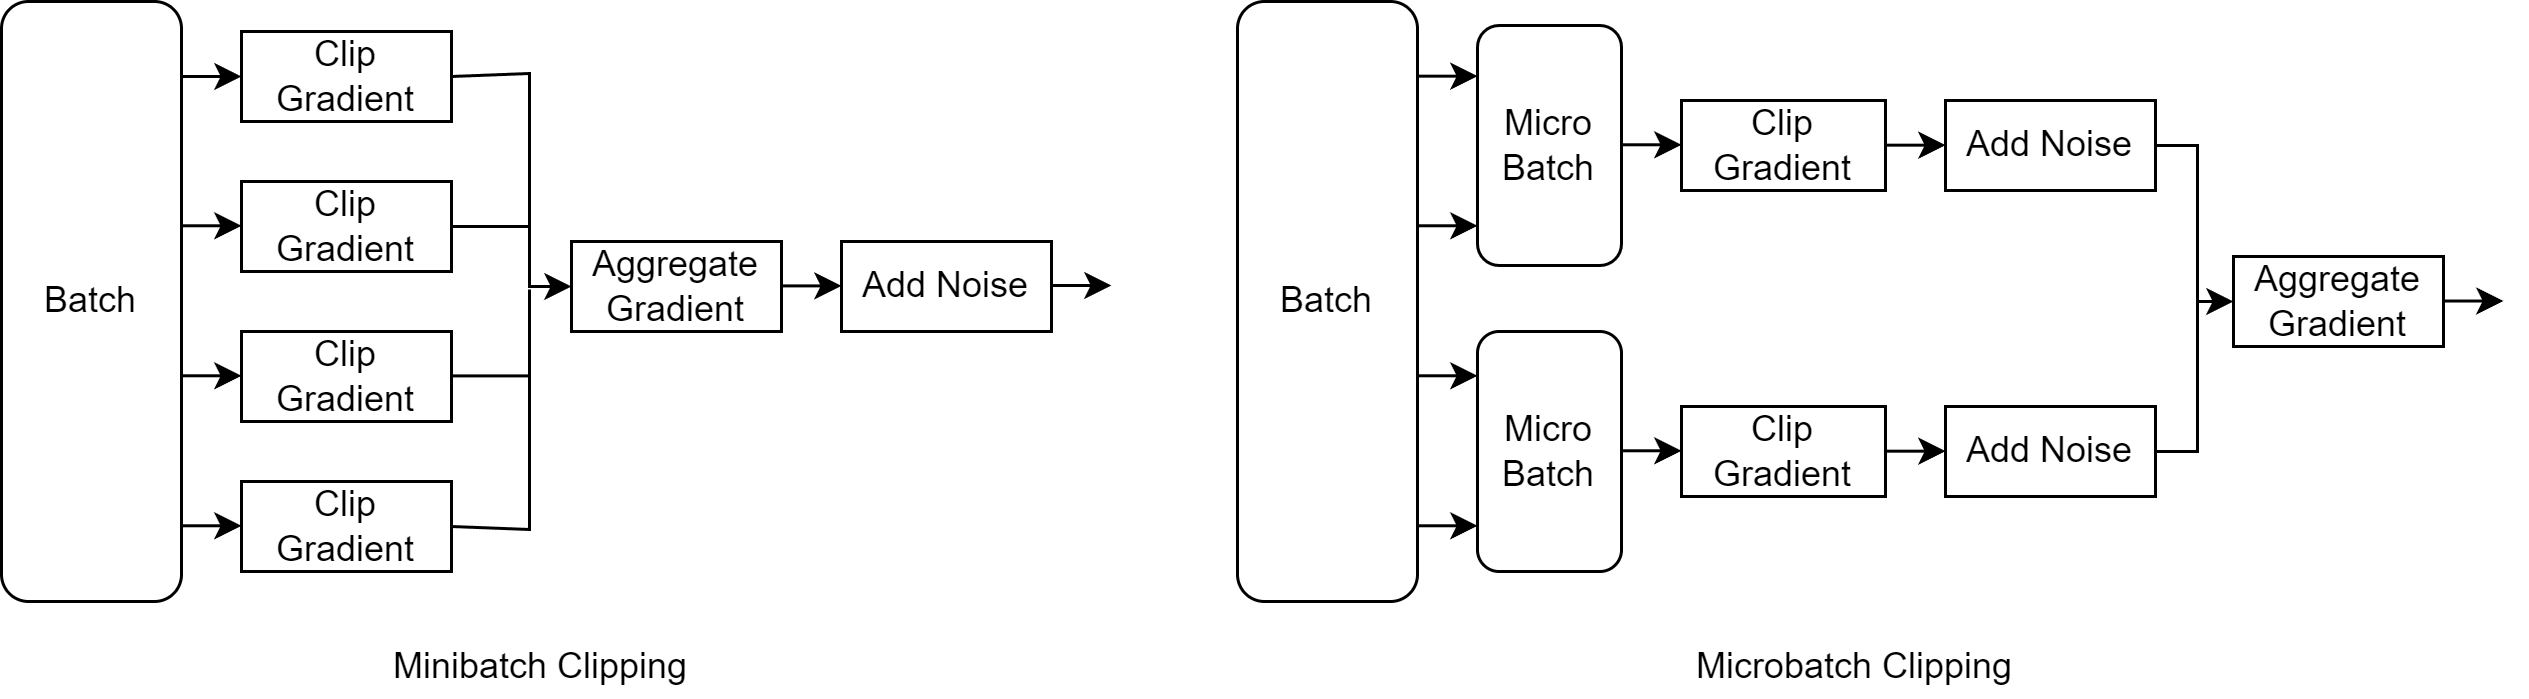
\includegraphics[width=1\linewidth]{submissions/submission5/figs/mini vs micro.png}

   
   \caption{Minibatch Clipping vs Microbatch Clipping}\label{FigDiff}
   \label{minibatchvsmicrobatch}
\end{figure} 

To combat the high memory and computational demands of DP-SGD, several works investigated solutions that ease the cost of DP-SGD, especially in the contest of large-scale models.  McMahan et al.~\cite{RefWorks:RefID:45-mcmahan2018learning} modified federated learning techniques for DP-SGD and distributed the training process to different mobile devices that share the same model. Dupuy et al.~\cite{RefWorks:RefID:43-dupuy2022efficient} proposed another technique for group-wise clipping involving the use of GPUs. Since DP-SGD is computationally expensive because each batch requires its own gradients, these batches can instead be divided into micro-batches and assigned their own GPU. This reduces the computational cost of computing the overall gradient as the work is divided between the GPUs. %Furthermore, scaling and noise addition is done independently by each micro-batch, where once each micro-batch finishes its computation, their clipped noisy gradient and the model aggregates all of the to return an overall gradient. 


\subsection{Group-wise Clipping}

%Although these techniques offers valuable solutions for large-scale training, the focus on these papers are not on improving the efficiency of DP-SGD. Author 
He et al.~\cite{RefWorks:RefID:39-he2022exploring} investigated group-wise clipping for its memory and processing advantage compared to traditional flat clipping, regardless of the size of the model. Two group-wise clipping techniques were considered: per-layer clipping and per-device clipping.

\subsubsection{Per-layer Clipping}
\begin{figure}[h]
\centering
         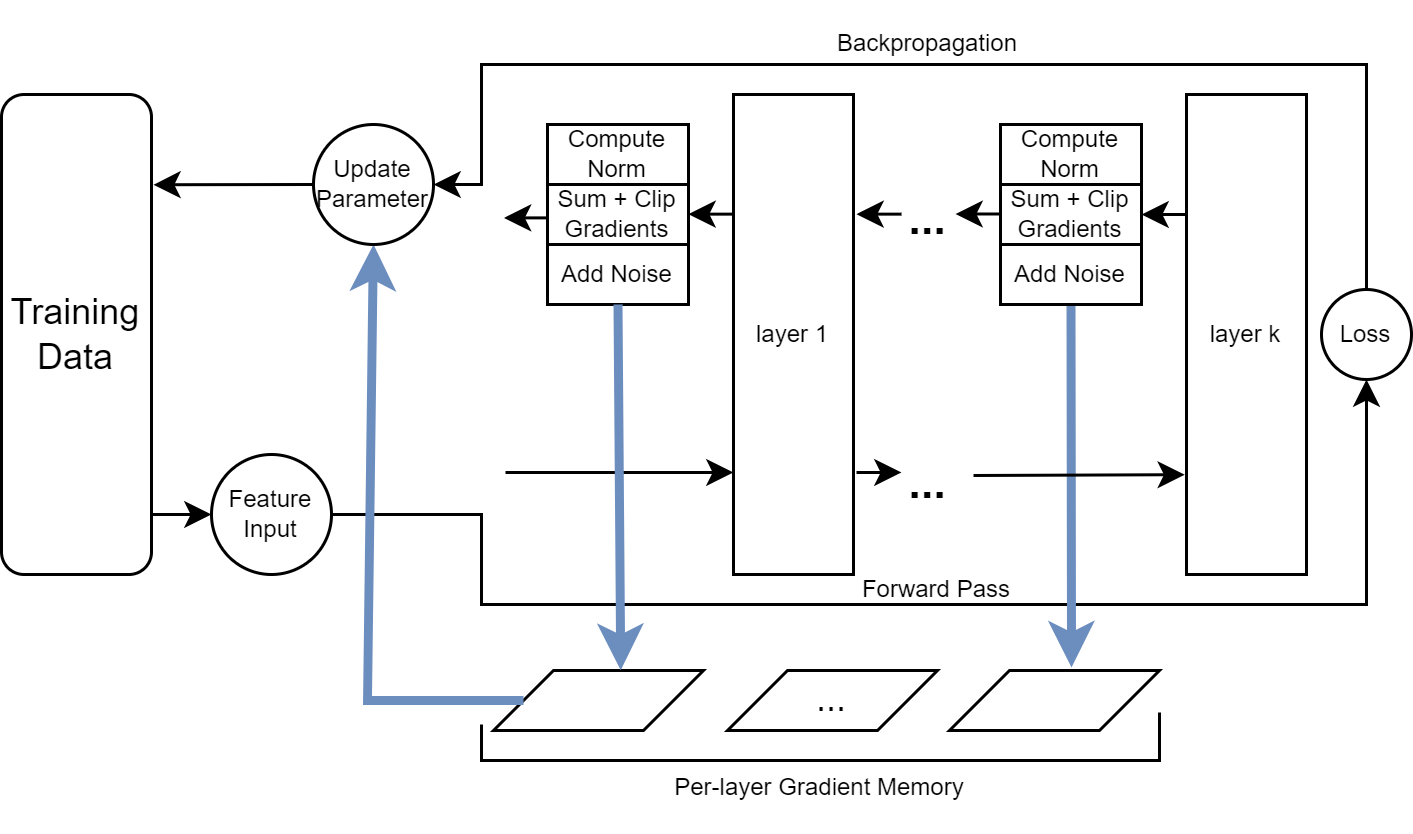
\includegraphics[width=1\linewidth]{submissions/submission5/figs/Per Layer Clipping.png}      
   \caption{Per-layer Clipping}\label{FigDiff}
   \label{perlayerclipping}
\end{figure} 
In per-layer clipping, per-example gradients of each layer in a neural network are clipped separately. Parameters of a neural network are grouped together and each of the $K$ layers in the network is prescribed its own clipping threshold, $C_k$. This brings the main advantage of per-layer clipping, in which gradient clipping for a particular layer can be done as soon as the backpropagation returns the output gradient of that layer, allowing clipping to be done together with backpropagation, as opposed to flat clipping which requires backpropagation to completely finish first. Additionally, the process of summing and clipping of the per-example gradient can be combined as soon as the input activation, output gradients and per-example gradient norms are known. Figure~\ref{perlayerclipping} shows the entire training cycle and how each layer performs its gradient computation, as well as how each layer's gradients are stored separately to perform the parameter updates corresponding to each individual layer. Besides the computational advantage, this method does not require instantiating the per-example gradients in memory, and instead can be computed as needed. This technique is referred to as ghost clipping~\cite{RefWorks:RefID:44-li2022large}. 
%The extra computations for the gradient norm and scaling are often cheap, making this method of private training not just memory-efficient but also time-efficient compared to the non-private counterpart for small to moderate scale workflow.

However, even though a computational advantage is noticed for per-layer clipping, utilizing a fixed clipping threshold for each layer ends up making the model perform worse compared to the traditional flat clipping method in certain scenarios. Observations during training reveal significant fluctuations in the magnitudes of per-layer gradients throughout the process. While gradients may initially be uniformly low, they tend to increase notably for layers closer to the input as training progresses. It is suggested that employing a fixed layer-wise clipping threshold eliminates the structural relationship between gradients of different layers, introducing an additional source of bias on top of the inherent bias associated with flat clipping techniques. As a solution to the performance problems of fixed per-layer clipping, adaptive clipping thresholds can alleviate the structural bias that comes with clipping gradients of different layers separately. In this case, the adaptive clipping technique focuses a quantile estimation, as discussed in Section~\ref{sec:adaptation}.

\subsubsection{Per-device Clipping}

Another group-wise clipping technique explored in~\cite{RefWorks:RefID:39-he2022exploring} is per-device clipping. The main motivation for this method is to make use of larger/better pre-trained model as past works have shown using them improves the privacy-utility trade off. The problem is that size of the model makes it so that the model weights cannot be fit in a single device (GPU), making it a difficult computational problem. The solution to this problem revolves around pipeline parallelism popularly used in non-private training~\cite{RefWorks:RefID:50-huanggpipe:}. The model is first partitioned into consecutive blocks/layers which is then assigned to its own accelerator (i.e., GPU). Forward computation is performed on micro-batches (split mini-batches) that chain together the local computations done on each model partition by communicating activation outputs between the GPUs. Backpropagation reverses this process but on each GPU, and intermediate forward computations are performed to reduce peak memory usage. Furthermore, parallel computation is enabled across GPUs to reduce overall training time. Once all micro-batches finish their forward and backward computation, SGD performs its parameter updates, and the GPUs are synchronized.

Since flat clipping requires computing per-example gradient norms in order to get the scaling factors for computing gradients, it becomes necessary to have additional communication between devices to get the per-example norms of their local gradients. This ends up adding extra overhead to the pipeline parallelism process~\cite{RefWorks:RefID:39-he2022exploring}. There are three potential approaches to reduce communication, however both of them result in non-trivial slowdowns and increased complexity in the implementation. The first approach is to synchronize all the devices after the full backward pass is finished for each micro-batch. This allows each device to have the same gradient norms for computing the clipping scaling factor, but it ends up requiring as many synchronization steps as the amount of micro-batches in a mini-batch, which further reduces efficiency when micro-batches are large. 
%Although this is executing the primitives themselves are not costly, the disruption caused to the pipeline by the frequent calls ends up becoming costly. The devices ends up needing to perform one of three options; the first is to keep the unclipped local per-example gradients for the micro-batches, and to keep being idle until micro-batch synchronization is called to avoid any memory errors, which is a problem initself as resources are being wasted keeping the devices idle. 
The second option is to offload the unclipped local per-example gradients to the CPU, and to transport them back during synchronization. The problem here is the slow CPU-GPU data transfer rates ends up being costly. The last option is to re-materialize the local per-example gradient during synchronization, which ends up being costly as it requires a second  backpropagation step to be performed. 
%As seen, all the options incurs some kind of performance loss.

%As an alternative, a new per-device clipping scheme is proposed where each device is assigned it's own clipping threshold for clipping the per-example gradients of the hosted model piece. Using the equal budget strategy discussed earlier, the noise level added to the gradients in each device is independent of each other, which means no extra communication is necessary.


\subsection{Quantifying Memory Requirements}
\begin{figure}[h]
\centering
    \subfloat [Per-layer Clipping\label{fig:subfigA}] {
        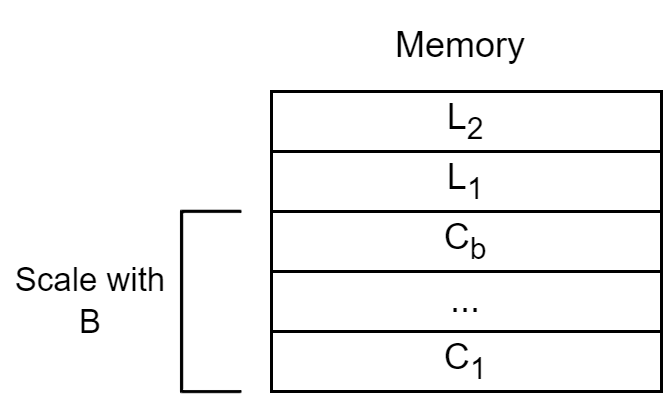
\includegraphics[width=0.4\linewidth]{submissions/submission5/figs/PerLayer.png}}
    \qquad
    \subfloat[Mini-batch Clipping\label{fig:subfigB}]{
          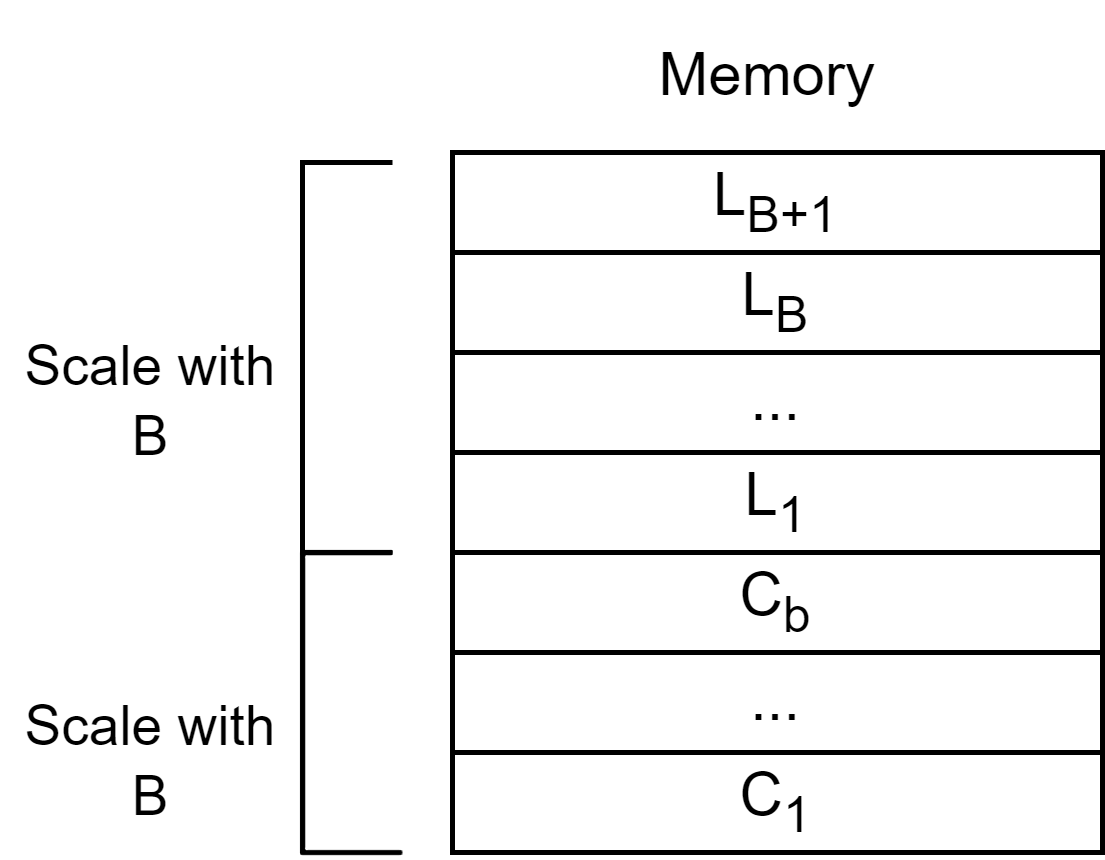
\includegraphics[width=0.4\linewidth]{submissions/submission5/figs/Minibatch.png}}    
   
   \caption{Per-layer Clipping Memory vs Mini-batch Clipping Memory}\label{FigDiff}
   \label{ClippingMemory}
\end{figure} 
Knowing the different ways clipping can be performed, it is important to quantify how much memory is required by each technique. Yousefpour et. al.~\cite{RefWorks:RefID:51-yousefpouropacus:} estimated the memory requirements in a per-example setting that uses the minibatching technique as follows:
\[ \text{M}_\text{non-DP}=bC+2L\]   
\[ \text{M}_\text{DP}=bC+(1+b)L\]
where $L$ is the number of trainable parameters with each one being of size $1$, $C$ is the size of the features, label, and model output for a single data point, and $M$ is the total memory usage for one forward and one backward pass on a batch of size $b$. The labels and outputs for $b$ data points are expected to occupy memory of size $bC$ and the model itself occupies memory of size $L$. In a non-private setting, the gradients are expected to occupy an additional memory of size $L$, meanwhile, for a private setting, the gradients are expected to occupy a memory of size $bL$ due to the need to store per-sample gradients. If the batch size is greater than or equal to 1, it's possible to get an estimate of how much memory private training requires compared to non-private as a ratio of the number of trainable parameters and the size of the model input/outputs. This is given as:
\[
\frac{\text{M}_\text{DP}}{\text{M}_\text{non-DP}} = \begin{cases} 
\frac{bC+(1+b)L}{bC}=1+\frac{L}{C}, & \text{if } L/C<<b \\
\frac{2+b}{3}=\frac{b}{3}, & \text{if } L/C=b \\
\frac{1+b}{2}=\frac{b}{2}, & \text{if } L/C>>b 
\end{cases}
\]


He et. al.~\cite{RefWorks:RefID:39-he2022exploring} compared the memory requirements between the per-layer clipping and the approach in~\cite{RefWorks:RefID:51-yousefpouropacus:} and found that per-layer clipping occupies a similar amount of memory as the non-private setting. This result is expected, given that the ghost clipping technique used in per-layer clipping eliminates the need to store per-sample gradients, making the memory requirement of storing the gradient independent of the batch size. This means that the traditional mini batching technique would require double the memory size compared to per-layer clipping, as traditional mini batching scales with the batch size twice, as opposed to only once with per-layer clipping. Figure~\ref{ClippingMemory} shows a comparison between the scaling factor with the batch size in terms of memory for per-layer clipping and mini-batch clipping. As an example, assume $L$ and $C$ both uses a memory unit of size $1$, and training uses a batch size of $100$. Using the equation above, we can estimate the memory required for traditional mini batch clipping with per-sample gradients to be $201$. Meanwhile, for per-layer clipping, we would need a memory block of size $102$ only. The difference will keep growing bigger with larger batch size, especially when we consider private training of large-scale models that require the use of multiple GPUs.
